\chapter{Estrategia de resolución}

En este capitulo se presenta el algoritmo desarrollado, su estructura, parámetros y configuración. 

Se comienza explicando la librería Malva utilizada para el desarrollo del algoritmo y la arquitectura especifica que se realizo para resolver el problema.

\section{Por que usar algoritmo genéticos?}
El problema de sincronización de semáforos es NP-Hard y 
no existe (hasta el momento) un método determinístico que lo
resuelva, se buscará mediante algoritmos evolutivos llegar a
una configuración aceptable minimizando los tiempos de
espera de los automóviles, mejorando así la configuración
actual de los semáforos del corredor de Garzón.


\section{Arquitectura de la solución}

En el siguiente diagrama muestra la arquitectura propuesta para el problema.

\begin{figure}[H]
\centering
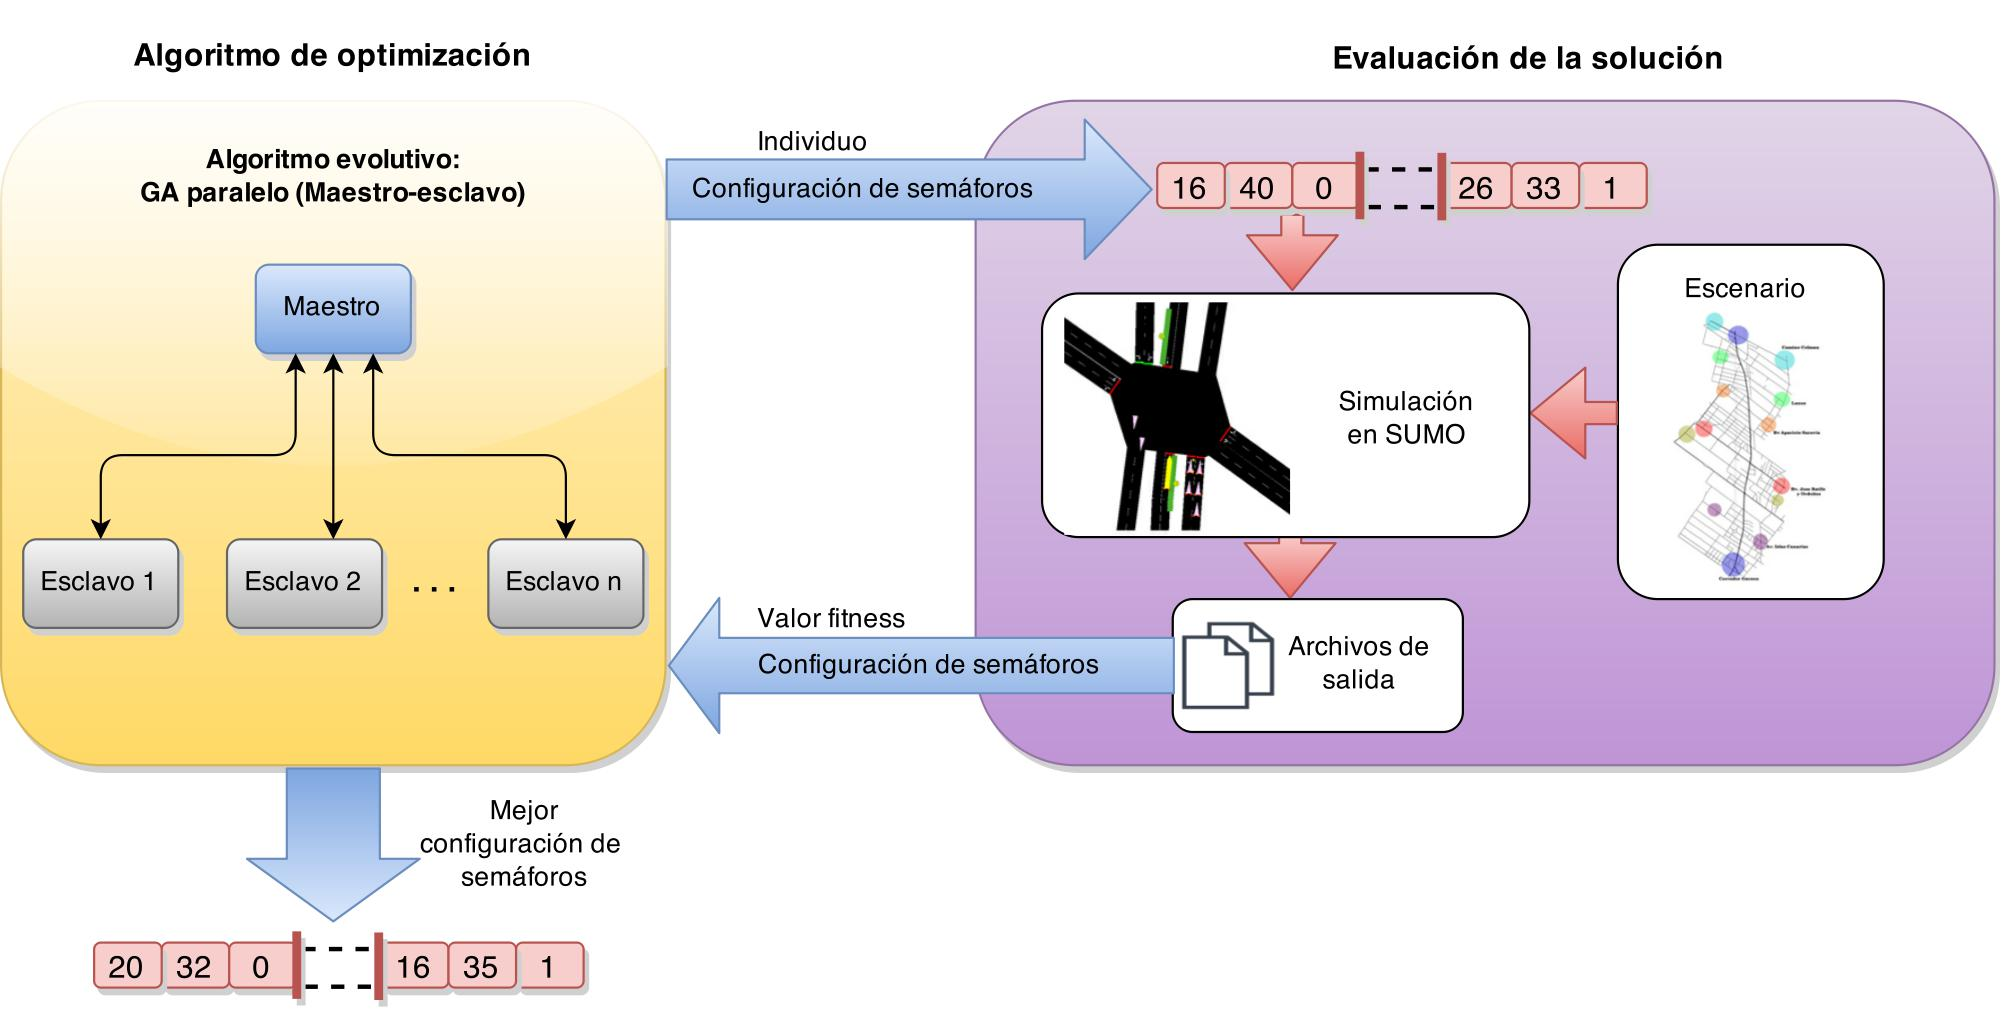
\includegraphics[width=0.7\linewidth]{Figures/arquitectura1}
\caption{Arquitectura del algoritmo}
\label{fig:arquitectura1}
\end{figure}


Malva se utiliza para la implementación del algoritmo, en cada evaluación de la función de fitness se realiza un llamado al simulador SUMO. 

El simulador genera archivos con información sobre la simulación que son usados por el algoritmo para determinar el fitness.

Luego los archivos son procesados por el algoritmo para extraer los datos útiles necesario para la función de fitness.







\section{Librería Malva}

\citep{Malva} surge como una variante del proyecto \citep{Mallba}. Propone la actualización, mejora y desarrollarlo como un proyecto de código abierto colaborativo.  Su objetivo es proveer de varios esqueletos de  heurísticas de optimización que puedan ser utilizados y extendidos de manera fácil y eficiente.

Los esqueletos se basan en separar dos conceptos: El problema concreto que se quiere resolver y por otro lado el método utilizado para resolverlo. Por tanto un esqueleto se puede ver como una plantilla genérica que se instancia para resolver un problema particular, manteniendo todas las funcionalidades genéricas.

Utiliza el lenguaje c++ dado su alto nivel, modularidad y flexibilidad. Los esqueletos se ofrecen como un conjunto de clases requeridas que son las que el usuario deberá modificar para adaptarlo a su problema y las provistas. que incluyen todos los aspectos internos del esqueleto y on independientes del problema particular. Entre los algoritmos provistos se encuentra el de Algoritmos genéticos y \citep{CHC}.


\newpage

\section{Especificación del Algoritmo Genético utilizado}
Se utiliza el algoritmo genético proviso por la librería  Malva  llamado NewGA al cual se le realizan algunas modificaciones para que se ejecute en paralelo.


Resumen de las características:
\begin{itemize}

\item Algoritmo paralelo: Utiliza el método maestro esclavo para que en cada iteración el maestro genere un hilo para cada ejecución  de la función fitness y luego espere a la terminación de todos los hilos para consolidar los datos. 
\item Función Multiobjetivo: Se intenta optimizar tanto la velocidad promedio de vehículos como de ómnibus teniendo cada uno un peso especifico.
\item Representación del cromosoma: Es un vector de números reales que representan los tiempos de los semáforos.
\item Cruzamiento y mutación: Se utiliza una variante del cruzamiento por un punto especifico para nuestro caso así como para la mutación.
\item Selección y reemplazo: Reemplaza padres por hijos, la selección de los padres se realiza por el método de torneo de 3 individuos, y la selección de hijos por el método de ruleta.

\end{itemize}

más adelante se realizara el ajuste paramétrico para determinar tanto el tiempo de simulación, criterio de parada y tasas de cruzamiento y mutación optimas para el algoritmo.

El siguiente esquema muestra el algoritmo utilizado. \citep{MalvaAlgGenetico}

 
\begin{algorithm}[H]
	\caption{Algoritmo Genético de Malva}
	\label{alg:algoritmo_genetico_malva}
	\begin{algorithmic} [1] 
		{
			\STATE \texttt{t} = 0
			\STATE {Inicializo( P(t))}
			\STATE {Evaluar estructuras en ( P(t))}			
			\WHILE {\text{No termine}}
			\STATE \texttt{t}++		
			\STATE {Seleccionar C(t) de P(t-1)}	
			\STATE {Recombinar estructuras en C(t) formando C'(t)}				
			\STATE {Mutar estructuras en C'(t) formando C''(t)}		
			\STATE {Evaluar estructuras en C''(t) generando un hilo de ejecucion por cada una}					
			\STATE {Consolidar valores de la evaluacion}								
			\STATE {Reemplazar P(t) de C''(t) y P(t-1)}								
			\ENDWHILE
		}
	\end{algorithmic}

\end{algorithm}




 

\subsection{Representación del cromosoma}

Se explican algunas definiciones necesarias para comprender la representación.

Cruce: Es el lugar de intersección de dos o más vías de circulación.
Fase: Es la configuración de las luces de los semáforos en un determinado cruce.

El  cromosoma  se  va  a  agrupar  lógicamente  en  cruces siendo el valor de cada gen el tiempo que demora una
fase de un cruce, además se agrega para cada cruce un número que representa en que fase comienza el semáforo. 
Por tanto el tamaño del cromosoma depende tanto de la cantidad de cruces como la cantidad de fases de cada uno.

En la representación se omiten las luces amarillas ya que no modifican los tiempos reales del paso de vehículos.
 
Es  importante que el algoritmo no genere soluciones inviables por lo que no debe modificar la combinación de luces de cada fase evitando combinaciones de luces erróneas. Por tanto tanto la modificación se realizara solo en el valor que indica el comienzo de fase y en los tiempos relacionados.

\begin{figure}[h]
\centering
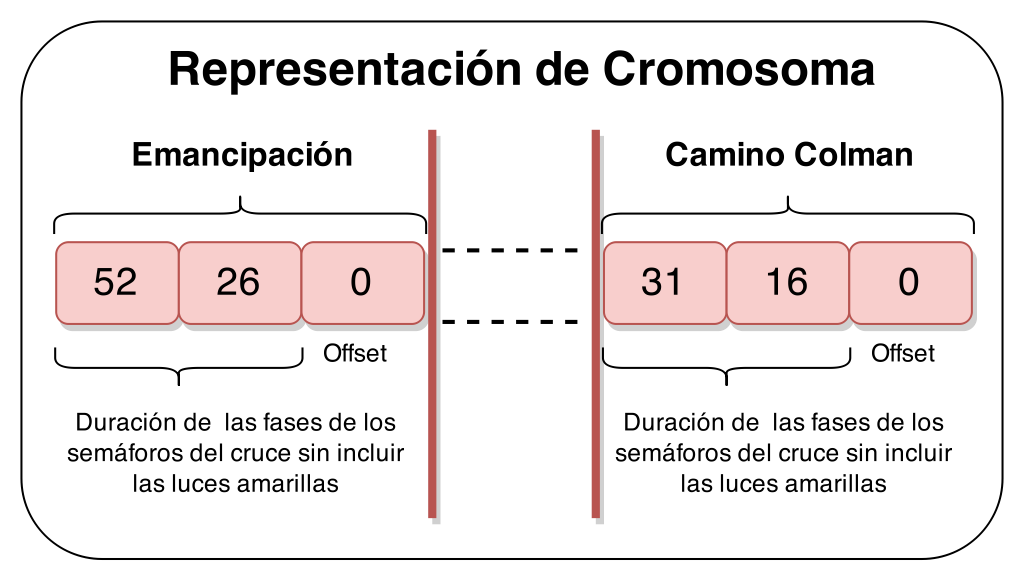
\includegraphics[width=0.7\linewidth]{Figures/cromosoma1}
\caption{Cromosoma de 2 cruces}
\label{fig:cromosoma1}
\end{figure}

En la siguiente figura vemos la representación de los archivos de simulación que nos provee SUMO para el cromosoma anterior, donde vemos como se representan las fases por ejemplo el texto “GGGGrrGGGGrr” demora 52 segundos. “G” es Verde, “r” es Rojo e “y” es Amarillo. El offset indica el inicio de la fase.

\begin{figure}[h]
\centering
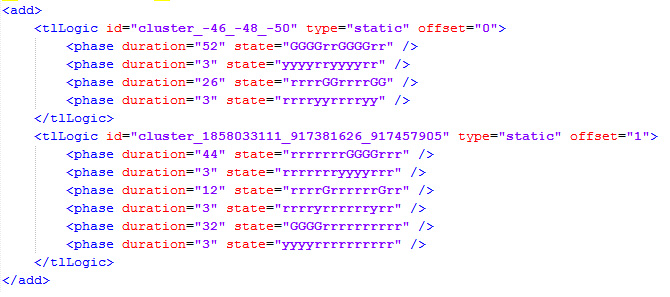
\includegraphics[width=\linewidth]{Figures/rep_sumo}
\caption{Representación de Sumo}
\label{fig:rep_sumo}
\end{figure}


\subsection{Inicialización}

Para la inicialización de la población se toma como referencia
la configuración obtenida con los datos in-situ, luego para cada
cruce se hacen variar las duraciones de las fases de manera aleatoria entre un rango de  5 a 60  segundos  (valores configurables)
además la fase inicial se elige aleatoriamente entre la cantidad de fases del cruce (se cuentan las luces amarillas).

\subsection{Función fitness}
La evaluación de un individuo se realiza generando un archivo con la configuración de los semáforos en base a su cromosoma y ejecutando el simulador SUMO utilizando esta configuración para luego obtener los tiempos necesarios para calcular el fitness.
Al ser una función multiobjetivo los datos que extraemos son la velocidad promedio de los ómnibus y la velocidad promedio del resto de los vehículos.

Esta es la formula de fitness donde x e y indica el peso que le podemos especificar a la función.

f = x.vb + y vv


\subsection{Operador de Cruzamiento}
Se  utilizará cruzamiento  de  un  punto,  implementado
específicamente  para  el  problema,  seleccionando  el  intervalo
entre 2 cruces como punto de corte, por tanto si un tramo del corredor tiene un buen comportamiento esta propiedad lo mantendrá.


\subsubsection{Operador de Mutación}
La  mutación también fue  implementada  específicamente para
el problema, utilizaremos dos tipos de mutación:
\begin{itemize}

\item Mutación de duración de fase: para cada fase de cada cruce se
hace variar su duración sumando o restando una cantidad dada
de segundos entre un rango determinado con una probabilidad
dada.
\item Mutación de inicio de cruce: se elige aleatoriamente una fase
con  la  cual  va  a  arrancar  inicialmente  el  cruce  con  una
probabilidad dada.

\end{itemize}

\section{Resumen}